\documentclass{beamer}
\usepackage[utf8]{inputenc}
\usepackage[T1]{fontenc}
\usepackage{hyperref}
\usepackage{graphicx}
\title{Update on the Dynamic Federation}
\date[ISPN ’80]{Technical Coordination Board}
\author[Euclid]{Frank Berghaus \href{mailto:berghaus@cern.ch}{\texttt{berghaus@cern.ch}}}

% --- Blocks ---
\setbeamertemplate{blocks}[default]

\usetheme{frank}

\begin{document}

\begin{frame}
\titlepage
\end{frame}


\begin{frame}
\frametitle{Review: What does DynaFed do?}
\begin{itemize}
\item Aggregates storage and metadata farms on-the-fly
\item Exposes standard protocols that support redirections and WAN data access
\item Creates (the illusion of) a unique namespace from a set of distinct storage or metadata endpoints
\item read and write support
\end{itemize}
\end{frame}

\begin{frame}
  \frametitle{Dynafed Namespace}
  \begin{figure}
      \centering
      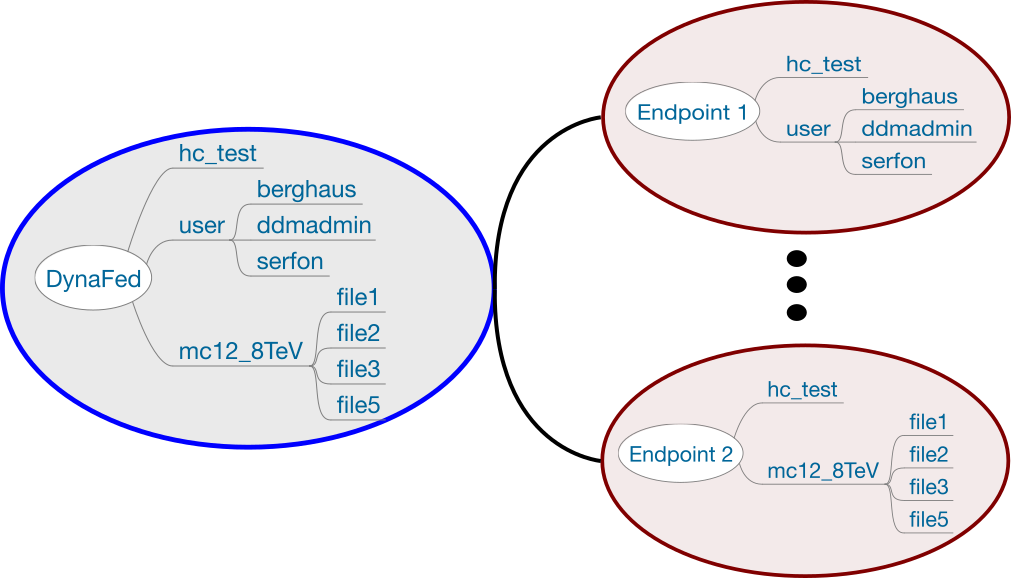
\includegraphics[width=\columnwidth]{dynafed-namespaces.png}
  \end{figure}
\end{frame}

\begin{frame}
  \frametitle{ATLAS Projects with DynaFed}
  \begin{itemize}
    \item At UVic: Rolf Seuster \& Marcus Ebert
    \item At CERN: Frank Berghaus
    \item At RAL: Alastair Dewhurst
    \item In Italy: Alessandro De Salvo
  \end{itemize}
  With lots of help from ADC and DDM!
\end{frame}

\end{document}
